%Results
\section{Descriptive statistics}
Before the experiment, the seeds were weighted in groups of ten, to see if there was a baseline difference between certain genotypes. Table \ref{tab:germination_percentage}, in the previous section, displays the measured weights.
After the completion of the experiment, the outliers were identified, and each plant was attributed a specific weight, following the protocol described in material and methods section. Those weights were used to compute the weighted mean and weighted standard deviation of the fresh and dry weight of the root system and the leaf system, as well as the area of the root system, for each plant. Dotplots representing those descritptive statistics as well as the data point are presented in figure \ref{fig:dotplot_all_variables}. The numerical values of these results are presented in table \ref{tab:summary_table_all_variables}, in appendix \ref{appendix:mean_std_table}.\\

Even though no clear conclusions can be made from these figures, we can see large variation of mean values between genotypes. Also, for some genotypes, the difference between tanks seem significant (e.g. genotype 15) while it's clearly not the case for some other (e.g. genotype 7). This implies that the tank and genotypes effects are significant. Overall the values of dry weights seem to have less variations than the fresh weights.

\begin{figure}
\centering
	\begin{subfigure}[t]{\textwidth}
		\centering
		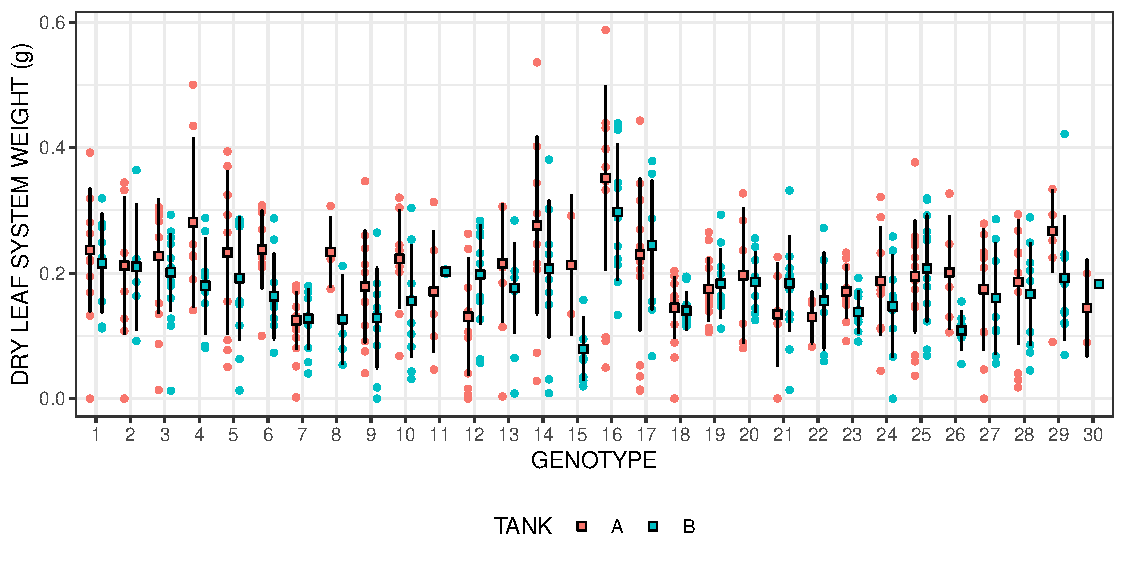
\includegraphics[width = \textwidth]{../../Figures/DRY_LS_summary_plot.pdf}
		\caption{Dry leaf weight ($DRY\_LS$)}
	\end{subfigure}

	\begin{subfigure}[t]{\textwidth}
		\centering
		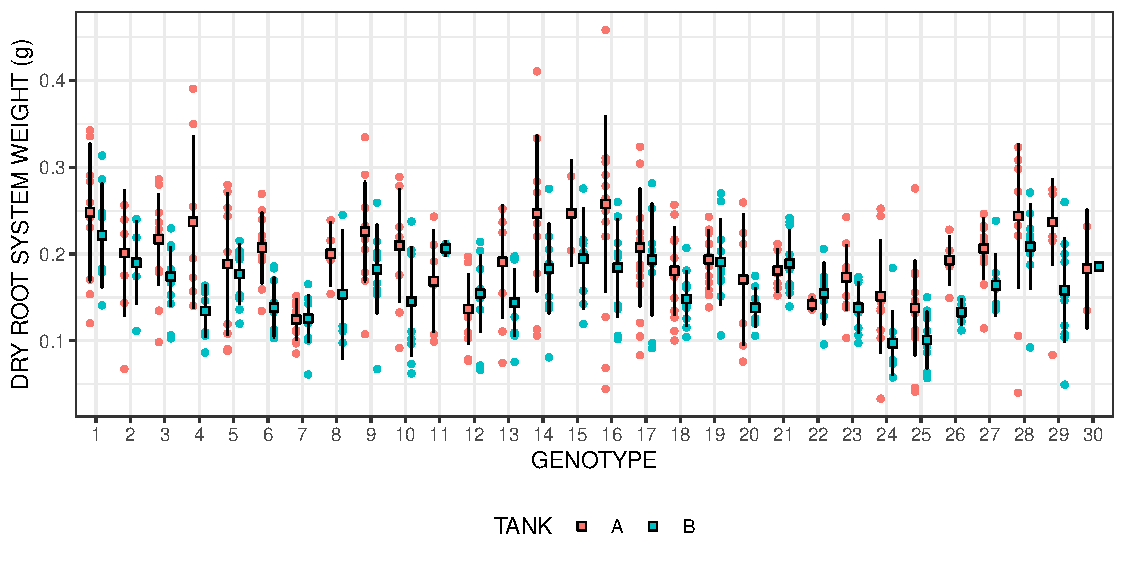
\includegraphics[width = \textwidth]{../../Figures/DRY_RS_summary_plot.pdf}
		\caption{Dry root weight ($DRY\_RS$)}
	\end{subfigure}
	\caption[Dotplot of the mean weight and associated standard deviation]{Dotplot displaying mean weight (\protect\emptysquare) and associated standard deviation (\protect\blackline), grouped by tanks for each variable.}
\end{figure}
\begin{figure}\ContinuedFloat
	\captionsetup[figure]{list=no}
	\begin{subfigure}[t]{\textwidth}
		\centering
		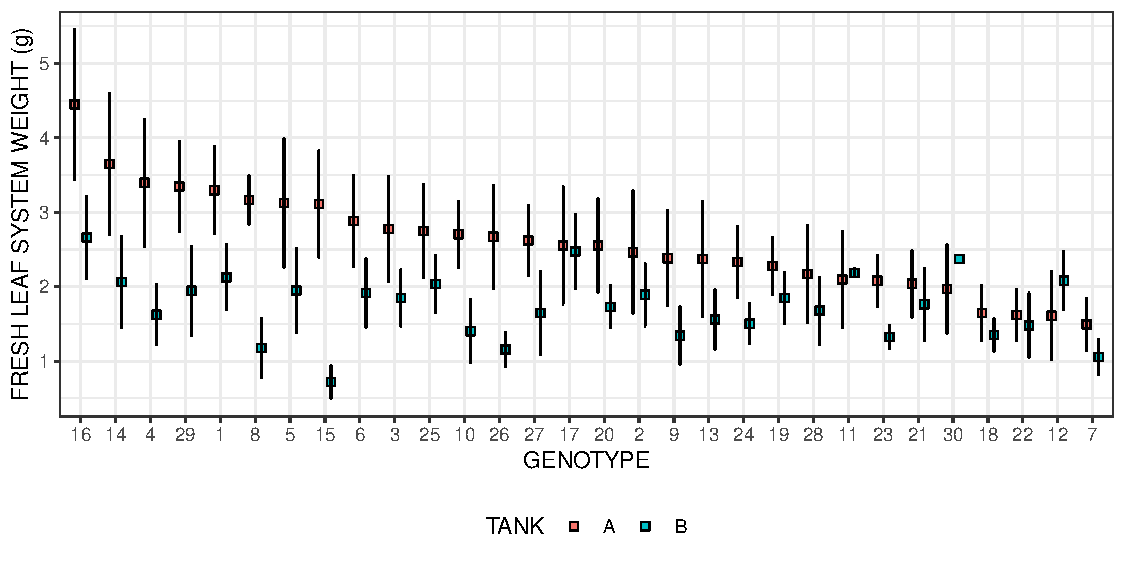
\includegraphics[width = \textwidth]{../../Figures/FRESH_LS_summary_plot.pdf}
		\caption{Fresh leaf weight ($FRESH\_LS$)}
	\end{subfigure}

	\begin{subfigure}[t]{\textwidth}
		\centering
		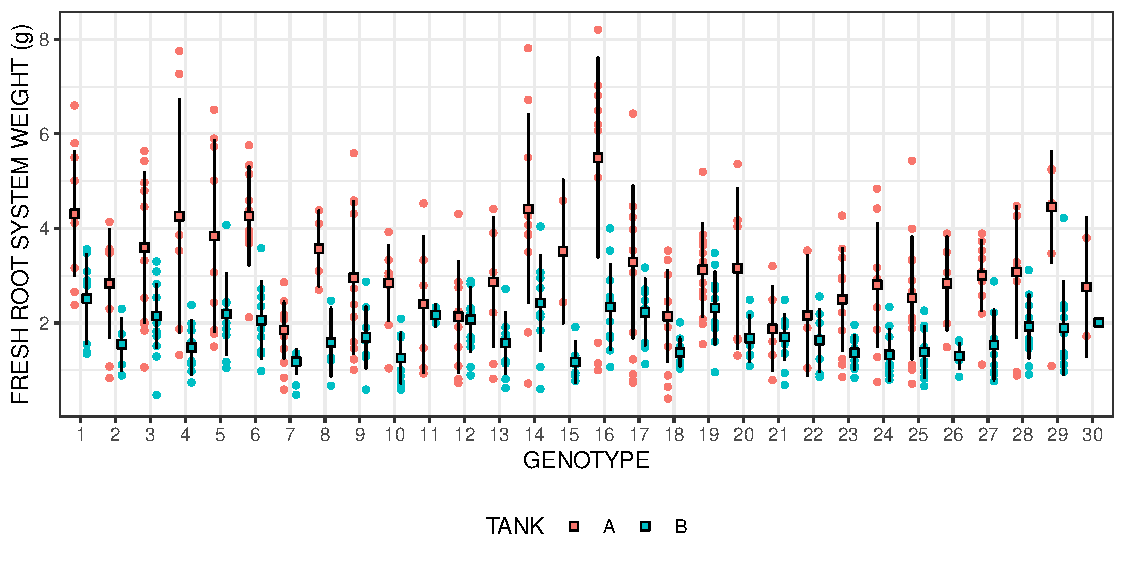
\includegraphics[width = \textwidth]{../../Figures/FRESH_RS_summary_plot.pdf}
		\caption{Fresh root weight ($FRESH\_RS$)}
	\end{subfigure}
	\caption[Dotplot of the mean weight and associated standard deviation]{Dotplot displaying mean weight (\protect\emptysquare) and associated standard deviation (\protect\blackline), grouped by tanks for each variable.}
	\label{fig:dotplot_all_variables}
\end{figure}

\section{SpATS analysis}
The SpATS model usually takes rows and columns coordinates as inputs for spatial position. Given that we have tanks (A and B), strips (from 1 to 99) and positions (from 1 to 5), we reshaped the data to give have the tank side by side and the 99 strips divided in two columns (to have a similar disposition to the one in the greenhouse). Figure \ref{fig:tank_disposition} shows the reshaping of the positions. This new display of the data allows us to see the difference between tanks more clearly and to visualize the variables' values as they were in the greenhouse.

\begin{figure}[hbtp]
	\centering
	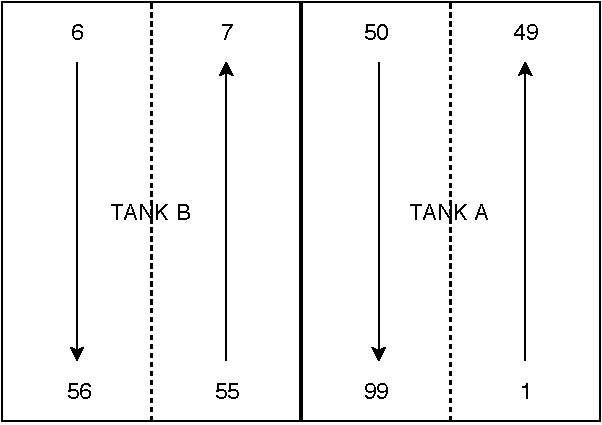
\includegraphics[scale = 0.7]{figures/TANK_repartition.pdf}
	\caption[Reshaping of the data table to fit the disposition of the greenhouse]{Reshaping of the data table to fit the 
	disposition of the greenhouse. The number indicates the original strip number.}
	\label{fig:tank_disposition}	
\end{figure}

The model was then fitted for the four weight variables, using the settings specified in the previous chapter. Table \ref{tab:spats_dimensions} presents the effective dimensions associated with the bivariate smooth surface components (see equation \ref{eq:full_bivariate_smooth_surface_model}) 
and their relative contribution to the fitted surface for each variable.
We see that the fresh weights exhibited a higher complexity in the structure of the spatial surface. This is reflected by the higher value of contribution for the smooth-by-smooth term ($f_{u, v}(\boldsymbol{u}, \boldsymbol{v})$), that accounts for almost 70\% in both variables. Besides this term, the main sources of variation are the linear (for the strips) by smooth (for the positions) term and the smooth trend along the strips term. It is not surprising to have more variation along the strips than along the positions given that there were 99 strips but only 5 positions.
Concerning the dry weights, the variation is more spread between all the components for both variables. This means that the variation in the data can be more easily attributed to the strips and positions of the plants. However, all the variables have components with zero value of $ED_{s}$\footnote{the actual values were not zero but it is denoted as such since they were inferior to $1 \times 10^{-15}$}, indicating that these terms were not necessary to model the spatial surface.\\

% Table generated by Excel2LaTeX from sheet 'Sheet2'
\begin{table}[htbp]
  \rowcolors{2}{gray!25}{white}
  \centering
  \caption[Effective dimensions of the SpATS model]{Model dimensions and effective dimensions (and percentage of the total of 
  the spatial components) of each spatial components for all variables. $ED_{\epsilon}$ represents the effective dimensions for 
  the residuals; $ED_{g}$, is the effective dimensions for the genotype and $H_{g}^2$ is the heritability. Here $\mathbf{v}$ 
  represents the columns, i.e. the position on the strip; and $\mathbf{u}$ represents the rows, i.e. the strip itself.}
    \begin{tabular}{lrrrrr}
    \toprule
    \begin{tabular}[b]{@{}l@{}}Model \\ components\end{tabular} & \multicolumn{1}{c}{Model} & \multicolumn{1}{l}{FRESH\_LS} & \multicolumn{1}{l}{FRESH\_RS} & \multicolumn{1}{l}{DRY\_LS} & \multicolumn{1}{l}{DRY\_RS} \\
    \midrule
    $f_{v}(\mathbf{v})$ & 6     & 0 (0,00\%) & 0 (0,00\%) & 0 (0,00\%) & 0 (0,00\%) \\
    $f_{u}(\mathbf{u})$ & 100   & 0,8 (8,73\%) & 2,26 (14,10\%) & 1,02 (17,26\%) & 1,8 (17,26\%) \\
    $\boldsymbol{u} \odot h_{v}(\boldsymbol{v})$ & 6     & 1,84 (19,95\%) & 2,63 (16,40\%) & 1,47 (24,77\%) & 2,54 (24,77\%) \\
    $\boldsymbol{v} \odot h_{u}(\boldsymbol{u})$ & 100   & 0,24 (2,56\%) & 0 (0,00\%) & 1,09 (18,36\%) & 0,49 (18,36\%) \\
    $f_{u, v}(\boldsymbol{u}, \boldsymbol{v})$ & 150   & 6,33 (68,76\%) & 11,16 (69,50\%) & 2,35 (39,62\%) & 0,08 (39,62\%) \\
    Total & 362 & 9,21 (100\%) & 16,15 (100\%) & 5,93 (100\%)& 4,91 (100\%)\\
    \midrule
    $ED_{\epsilon}$ &       & 466.6 & 459,3 & 470,2 & 470,1 \\
    \midrule
    $ED_{g}$  & 30    & 21,02 & 22,58 & 21,38 & 22,98 \\
    $H_{g}^2$ &       & 0,72  & 0,78  & 0,74  & 0,79 \\
    \bottomrule
    \end{tabular}%
  \label{tab:spats_dimensions}%
\end{table}%

Table \ref{tab:spats_dimensions} also presents the effective dimension of the genetic component ($ED_{g}$) which is quite similar across variables. This is reflected in the heritability values which are all around 75\%. However, it should be noted that the SpATS model tends to overestimate the heritability \parencite{rodriguez-alvarez_spatial_2016}. This means that a good part of the phenotypic variation can be attributed to genotypes.\\

Figure \ref{fig:spats_model_results} shows the raw data ($\mathbf{a}$), a graphical representation of the fitted spatial trend ($f(\boldsymbol{u}, \boldsymbol{v})$) ($\mathbf{b}$) and the spatially independent residuals $\boldsymbol{\epsilon}$ ($\mathbf{c}$) obtained from the SpATS package. While there are a lot of missing data, someone spatial trends still stand out. Just as predicted with the dotplot in the descriptive statistics section, weights in the B tank are lower than in the A tank. This is especially visible for the fresh weight, where the total weight range is greater than for the dry weights.\\

The inspection of the fitted spatial surfaces shows us that the trends have been captured by the SpATS model. An additional analysis of the residuals suggests that the spatial patterns have effectively been removed in all four variables by the tow-dimensional spline surface. However, some high data points still persists in the residuals, this is mainly due to the high variability of the weights in the raw data. In order to fully analyse the residuals, two additional diagnosis plots have been created: a lagplot to test for spatial independence and a normal distribution to test for the normality assumption. These plots are presented in appendix \ref{appendix:residuals}. Overall, the residuals seem to be independent and normally distributed, which confirms again that the spatial pattern has been well-captured by the model. Another interesting tool to evaluate the spatial independence is the variogram, presented in the previous chapter (section \ref{sec:arxar_model}). 
As said previously, if the model for spatial trend fits well, the variogram should be a horizontal plane \parencite{piepho_linear_2010}.\\

\begin{table}[ht]
\centering
\rowcolors{2}{gray!25}{white}
\caption{Individual variances of all the components of the SpATS model.} 
\begin{tabular}{lrrrr}
  \toprule
 & FRESH\_LS & FRESH\_RS & DRY\_LS & DRY\_RS \\ 
  \midrule
$\mathbf{c}_{g}$ & 0.171 & 0.262 & 1.27$\times 10^{-3}$ & 6.9$\times 10^{-4}$ \\ 
  $\mathbf{c}_{v}$ & 3.24$\times 10^{-3}$ & 5.08$\times 10^{-3}$ & 1.95$\times 10^{-7}$ & 8.47$\times 10^{-17}$ \\ 
  $\mathbf{c}_{u}$ & 1.86$\times 10^{-4}$ & 2.25$\times 10^{-5}$ & 2.42$\times 10^{-7}$ & 3.93$\times 10^{-8}$ \\ 
  $f_{v}(\mathbf{v})$ & 2.2 & 11 & 1.06$\times 10^{-4}$ & 0.265 \\ 
  $f_{u}(\mathbf{u})$ & 2.75$\times 10^{-5}$ & 5.36$\times 10^{-5}$ & 5.4$\times 10^{-8}$ & 1.55$\times 10^{-8}$ \\ 
  $\boldsymbol{u} \odot h_{v}(\boldsymbol{v})$ & 5.60$\times 10^{-52}$ & 1.76$\times 10^{-38}$ & 1.51$\times 10^{-52}$ & 1.44$\times 10^{-13}$ \\ 
  $\boldsymbol{v} \odot h_{u}(\boldsymbol{u})$ & 1.81$\times 10^{-9}$ & 4.83$\times 10^{-4}$ & 6.75$\times 10^{-10}$ & 1.43$\times 10^{-6}$ \\ 
  $f_{u, v}(\boldsymbol{u}, \boldsymbol{v})$ & 0.398 & 0.252 & 6.13$\times 10^{-5}$ & 7.13$\times 10^{-4}$ \\ 
  $\epsilon$ & 4.707 & 5.014 & 0.03364 & 0.01219\\
   \bottomrule
\end{tabular}
\label{tab:spats_variances}
\end{table}

Finally, another interesting result from figure \ref{fig:spats_model_results} is the comparison between the scales of spatial variations and residual variations, because they provide an idea of the relative importance of field trends for each variable. We see that for all variables, the scales of the residuals are about ten-fold the scales of the fitted surfaces. This is explained by the effective dimension of the residuals presented in table \ref{tab:spats_dimensions}. We see that, for all variables, those dimensions are much higher than the others. This means that the spatial variation was lower than the random variation, and even though spatial patterns were captured, much of the variation is still present in the residuals of the models. Given that the raw data present a high variability and a lot of missing values, we expected to have residuals with high variance (see table \ref{tab:spats_variances} for the variances linked to each component of the model).

\begin{figure}
	\begin{subfigure}[t]{\textwidth}
		\centering
		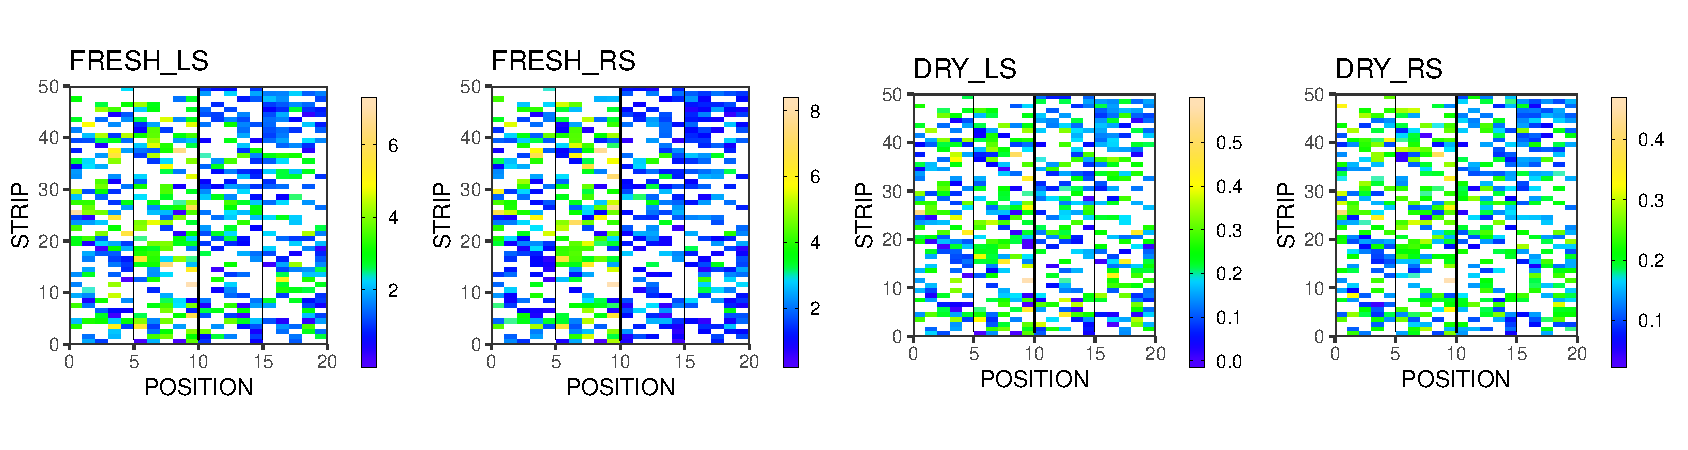
\includegraphics[width = \textwidth]{../../Figures/rawData_plot.pdf}
		\caption{Raw data}
	\end{subfigure}
	
	\begin{subfigure}[t]{\textwidth}
		\centering
		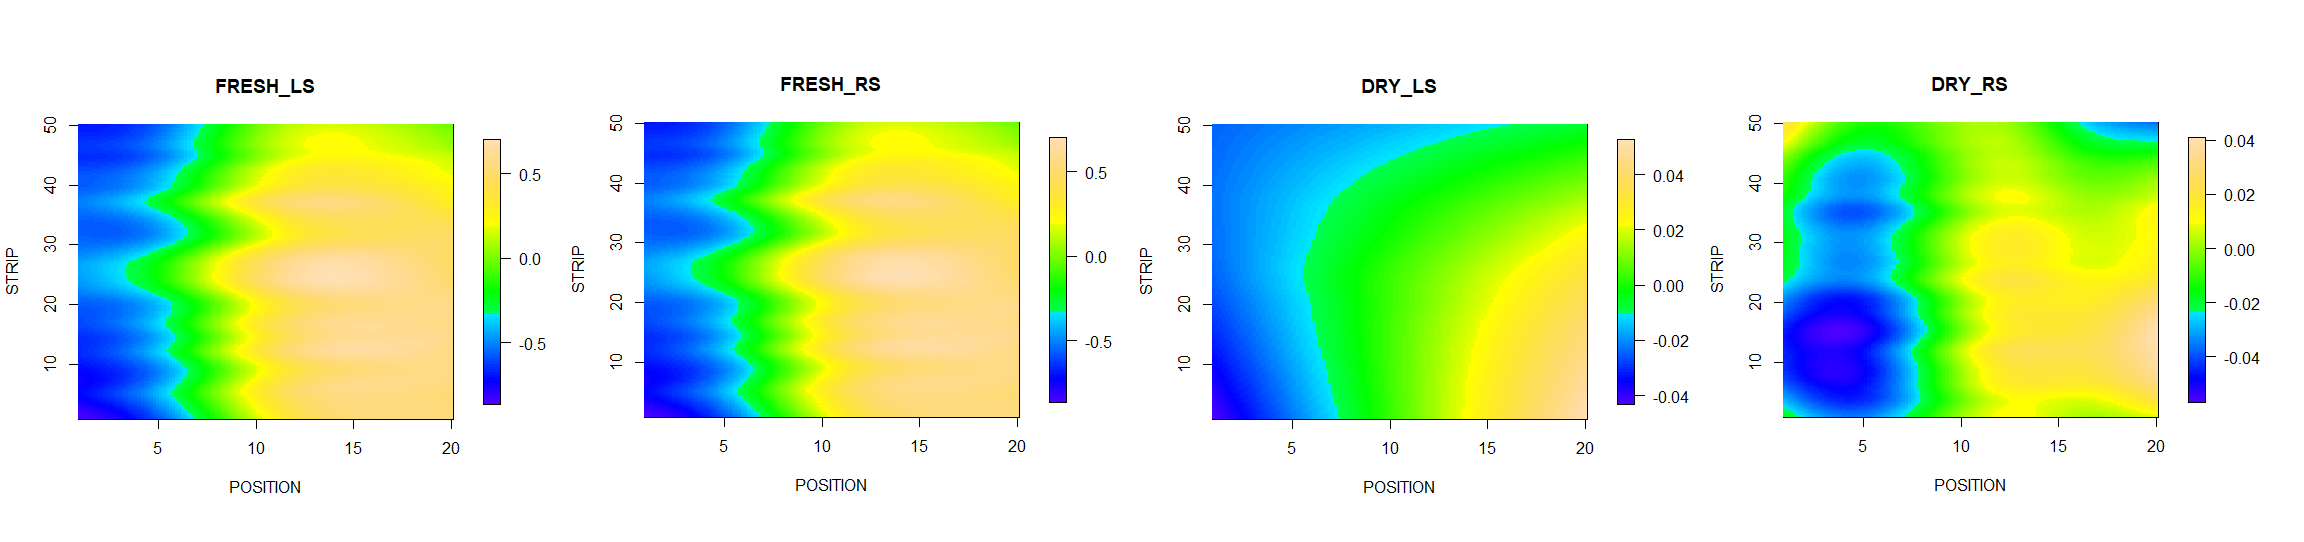
\includegraphics[width = \textwidth]{../../Figures/fitted.png}
		\caption{Fitted spatial trend}
	\end{subfigure}
	
	\begin{subfigure}[t]{\textwidth}
		\centering
		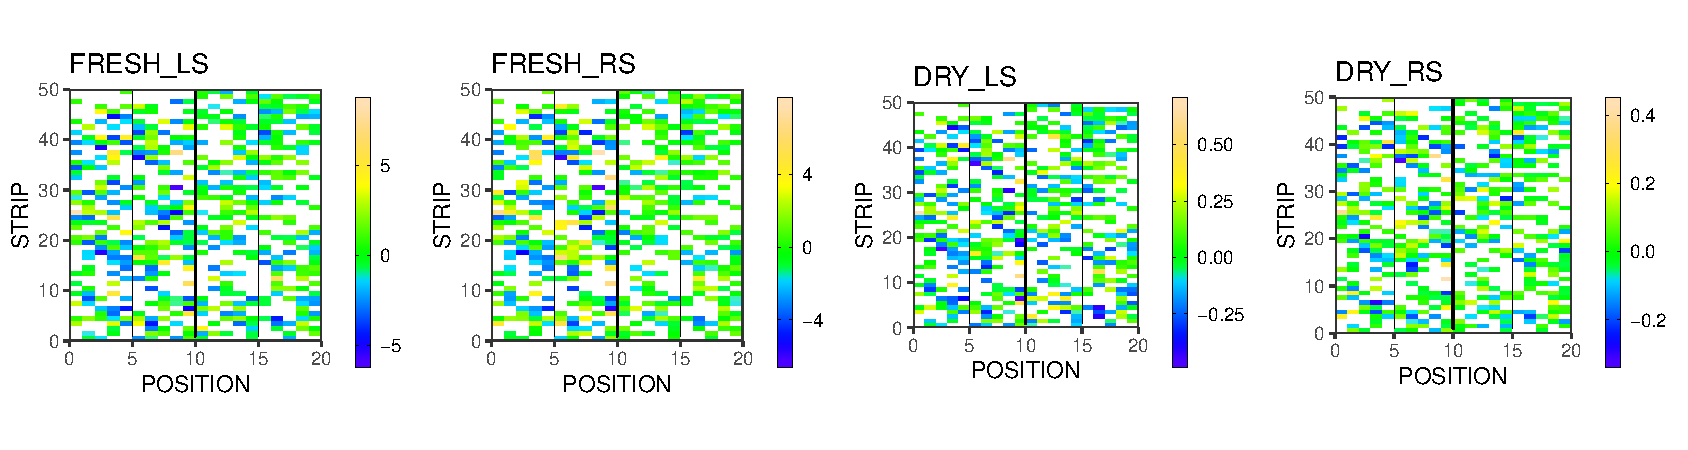
\includegraphics[width = \textwidth]{../../Figures/residuals_plot.pdf}
		\caption{Residuals' spatial plot}
	\end{subfigure}
	\caption{Raw data, fitted spatial trend and residuals' plot for each variable.}
	\label{fig:spats_model_results}
\end{figure}

\section{Standard spatial model analysis}
For the standard spatial model analysis, a baseline model, only considering a fixed effect for the tanks and random effects the rows, columns and the genotypes, was fitted for each of the four variables considered. Each model was then augmented by adding linear regression terms on the rows and columns and one of the following covariance structure:
\begin{itemize}
\item $AR(1)$ process along the rows or columns
\item $AR(1) \times AR(1)$ process
\item $LV$ process along the rows or columns
\item Superimposed row and column structure $LV + LV$
\item Separable process along the rows or columns $LV\otimes J$
\item Separable process along the rows and columns $LV \times LV$
\end{itemize}
At each step, the AIC and the Deviance were computed and the best model was selected using this criterion (a lower value is preferred). Table \ref{tab:selected_BSS_models} gives the structure of the final model for each variable. ...INTERPRETATION OF THOSE MODELS (similar or not ?). Then the variograms of the residuals were analysed to see if any leftover spatial pattern was still there. Figure \ref{fig:BSS_variograms} presents those variograms, ..INTERPRETATION.. + ANALYSIS of the residuals in the same way as the SpATS model.

\begin{table}[htbp]
  \rowcolors{2}{gray!25}{white}
  \centering
  \caption[Selected BSS models]{Best standard spatial (BSS) model selected for each of the four variables. All the models 
  contain an intercept and a fixed effect for the tank. $P$ represents a random effect for the positions (columns), $S$ a random effect for the strips (rows) and $n$ represent the spatially independent residuals.}
    \begin{tabular}{lr}
    \toprule
    Variable & \multicolumn{1}{l}{BSS} \\
    \midrule
    FRESH\_LS & $P + S + AR(1) + n$  \\
    FRESH\_RS &  \\
    DRY\_LS &  \\
    DRY\_RS &  \\
    \bottomrule
    \end{tabular}%
\label{tab:selected_BSS_models}
\end{table}%

%\begin{figure}
%
%\caption[Variograms for the four variables]{Variograms for the four variables.}
%	\centering
%	\includegraphics[width = \textwidth]{}
%\label{fig:BSS_variograms}
%\end{figure}

Table \ref{tab:BSS_variance_values} gives the value of the variance and correlation components for each spatial model.

% Table generated by Excel2LaTeX from sheet 'Sheet1'
\begin{table}[htbp]
\rowcolors{2}{gray!25}{white}
  \centering
  \caption{Add caption}
    \begin{tabular}{lrrrrrr}
    \toprule
    Variable & \multicolumn{1}{l}{$\rho_{s}$} & \multicolumn{1}{l}{$\rho_{p}$} & \multicolumn{1}{l}{$\sigma_{g}^{2}$} & \multicolumn{1}{l}{$\sigma_{\xi}^{2}$} & \multicolumn{1}{l}{$\sigma_{\varepsilon}^{2}$} &  \\
    \midrule
    FRESH\_LS &       &       &       &       &       &  \\
    FRESH\_RS &       &       &       &       &       &  \\
    DRY\_LS &       &       &       &       &       &  \\
    DRY\_RS &       &       &       &       &       &  \\
    \bottomrule
    \end{tabular}%
  \label{tab:BSS_variance_values}%
\end{table}%



\section{Model comparison}

% Table generated by Excel2LaTeX from sheet 'Sheet1'
\begin{table}[htbp]
\rowcolors{2}{gray!25}{white}
  \centering
  \caption{Comparison of the estimated TANK fixed effect for both models.}
    \begin{tabular}{clrrrr}
    \toprule
          &       & \multicolumn{1}{l}{FRESH\_LS} & \multicolumn{1}{l}{FRESH\_RS} & \multicolumn{1}{l}{DRY\_LS} & \multicolumn{1}{l}{DRY\_RS} \\
    \midrule
    \multirow{3}[1]{*}{Tank A} 
    		& SpATS & 2.952693 & 3.728238 & 0.21638755 & 0.2223098 \\
          	& BSS   &       &       &       &  \\
          	& $\Delta$ &       &       &       &  \\
    \multirow{3}[1]{*}{Tank B} 
    		& SpATS & 1.334286  &  1.144482  &  0.1621801 &  0.1522603 \\
          	& BSS   &       &       &       &  \\
          	& $\Delta$ &       &       &       &  \\
    \bottomrule
    \end{tabular}%
  \label{tab:tank_effect_model_comparison}%
\end{table}%


% Table generated by Excel2LaTeX from sheet 'Sheet1'
\begin{table}[htbp]
  \centering
  \caption[Comparison of both models in term of genetic variance and residual variance]{Comparison of both models in term of genetic variance and residual variance. $\Delta$ represents the absolute difference between the two variances. }
    \begin{tabular}{clrrrr}
    \toprule
          &       & \multicolumn{1}{l}{FRESH\_LS} & \multicolumn{1}{l}{FRESH\_RS} & \multicolumn{1}{l}{DRY\_LS} & \multicolumn{1}{l}{DRY\_RS} \\
    \midrule
    \multirow{3}[2]{*}{$\sigma^2_{g}$} & SpATS &       &       &       &  \\
          & BSS   &       &       &       &  \\
          & $\Delta$ &       &       &       &  \\
    \midrule
    \multirow{3}[2]{*}{$\sigma^2_{\varepsilon}$} & SpATS &       &       &       &  \\
          & BSS   &       &       &       &  \\
          & $\Delta$ &       &       &       &  \\
    \bottomrule
    \end{tabular}%
  \label{tab:sigma_model_comparison}%
\end{table}%

%\subsection{Performances}
%\subsection{Parametrization}
%\subsection{Modelling strategy}
